%
%PEN INSTRUgSetMapCTION
%
\documentclass[11pt,a4j]{jarticle}
%\pagestyle{empty}
\usepackage{amsmath}
\usepackage{amssymb}
\usepackage{epsfig}
\usepackage{color}
%\usepackage{txfonts}

\setlength{\topmargin}{-20mm}
\setlength{\oddsidemargin}{-15mm}
\setlength{\textheight}{255mm}
\setlength{\textwidth}{185mm}

%---------- 箇条書き -----------

\newenvironment{itemize2}%  
{%
   \begin{list}{$\bullet$\ \ }% 見出し記号/直後の空白を調節
   {%
      \setlength{\itemindent}{0pt}
      \setlength{\leftmargin}{3zw}%  左のインデント
      \setlength{\rightmargin}{0zw}% 右のインデント
      \setlength{\labelsep}{0zw}%    黒丸と説明文の間
      \setlength{\labelwidth}{3zw}%  ラベルの幅
      \setlength{\itemsep}{0em}%     項目ごとの改行幅
      \setlength{\parsep}{0em}%      段落での改行幅
      \setlength{\listparindent}{0zw}% 段落での一字下り
   }
}{%
   \end{list}%
}
%---------- 番号つき箇条書き -----------

\newcounter{enum2}
\newenvironment{enumerate2}{%
   \begin{list}%
   {%
      \arabic{enum2}.\ \,%  見出し記号/直後の空白を調節
   }%
   {%
      \usecounter{enum2}
      \setlength{\itemindent}{0zw}%  ここは 0 に固定
      \setlength{\leftmargin}{3zw}%  左のインデント
      \setlength{\rightmargin}{0zw}% 右のインデント
      \setlength{\labelsep}{0zw}%    黒丸と説明文の間
      \setlength{\labelwidth}{3zw}%  ラベルの幅
      \setlength{\itemsep}{0em}%     項目ごとの改行幅
      \setlength{\parsep}{0em}%      段落での改行幅
      \setlength{\listparindent}{0zw}% 段落での一字下り
   }
}{%
   \end{list}%
}
\setlength{\topsep}{0pt}
\setlength{\itemsep}{10pt}
\setlength{\parsep}{0mm}
\setlength{\itemindent}{50mm}

%\labelsep 20mm
%\labelwidth 50mm
%\leftmargin 100mm
\newcommand{\ExerciseTitle}[1]{%
  \begin{center}\Large
    \textbf{PEN マニュアル Q \& A} \qquad \texttt{#1}
  \end{center}%
}

\renewcommand{\baselinestretch}{1.0}

\begin{document}

\noindent
\begin{flushright}
{\small	2008/10/27}
\end{flushright}
\begin{center}
\begin{LARGE}
{\bf{図形描画のための関数群}}\\
\ \\
\end{LARGE}
\end{center}

  図形描画のための関数は以下の関数群から構成される。
\begin{itemize2}
  \item [(1)] 描画のためのウィンドウのオープン/クローズ関数 
  \item [(2)] 図形の属性を指定するための関数 
  \item [(3)] 図形を描画するための関数 
  \item [(4)] その他
\end{itemize2}

  図形は、一つのウィンドウ上に描画する。このウィンドウの大きさを指定し
て開くための関数として gOpenWindow()がある。 gCloseWindow()は閉じるた
めの関数であるが、この関数を呼び出すと描画ウィンドウが画面から消滅す
るので、通常この関数を使用することはない。 \\
  図形は、線分、折れ線などの{\bf{線図形}}、長方形、楕円、
多角形などの{\bf{面図形}}、
および、{\bf{文字図形}}からなる。 図形を描くには、原則として先に描画属性を指 
定しなければな らない。描画属性としては、線の太さ、線の種類、線の色等 
の線図形に適応されるもの、塗りつぶしの色等の面図形に適応されるもの、 
および、フォントの種類、フォントサイズ等の文字図形に適応されるものが 
ある。描画属性を指定しない場合は、予め定められた属性値が用いられ、一 
旦、設定した属性値は、同じ属性に対して新たに設定されるまで有効である。 
  図形を描画するための関数としては、線分の描画、長方形の描画、楕円の 
描画、円の描画、文字列の描画等の関数がある。 \\
\ \\
  以下、各関数について説明する。 \\
\ \\
{\large{
{\bf{
(1) 描画のためのウィンドウのオープン/クローズ関数
}}
}}
\begin{enumerate2}
\item {\bf{gOpenWindow(整数 w, 整数 h)}} \\
%   整数  w, h \\
       幅w、高さhの描画のためのウィンドウを開く。ウィンドウ 
       の位置は、画面の左上に固定される。 \\
\ \\
	   \hspace{10pt} $[$使用例$]$  幅400、高さ400のウィンドウを開く。 \\
           \hspace{55pt} gOpenWindow(400, 400)  \\

\item {\bf{gSaveWindow(文字列 filepath, 文字列 format)}} \\
%     文字列  filepath, format \\
     描画したウィンドウを保存する。
     保存形式(mode)はJPEGまたはPNGのどちらかを指定する。 \\
\ \\
	   \hspace{10pt} $[$使用例$]$  カレントディレクトリ(フォルダ)にウィンドウをpng型式でファイル名をabc.pngとして保存する。 \\
           \hspace{55pt} gSaveWindow(``./abc.PNG'', ``PNG'')\\

\item {\bf{gCloseWindow()}} \\
       描画のためのウィンドウを閉じる。
\end{enumerate2}
{\large{
{\bf{
(2) 図形の属性を指定するための関数
}}
}}
\begin{enumerate2}
\item {\bf{gSetLineColor(整数 r, 整数 g, 整数 b)}} \\
%   整数  r, g, b (値の範囲0-255) \\
   r, g, b の値の範囲は0-255。
       線の色属性を、赤の要素r、緑の要素g、青の要素bで指定する。
       初期値は黒(0, 0, 0)。\\
\ \\
	 \hspace{10pt}  $[$使用例$]$ 線の色を黄色に設定する。\\
         \hspace{55pt}     gSetLineColor(255, 255, 0) \\

\item {\bf{gSetLineShape(整数 type)}} \\
%   整数  type \\
      描画する線のタイプを変更。線を使用する全ての描画に影響。

      \begin{table}[!h]
      \begin{center}
      {\small{
      \begin{tabular}{l l}
        type=0のとき & 実線 (初期値) \\
        type=1のとき & 破線 \\
        type=2のとき & 間隔の狭い破線 \\
        type=3のとき & 一点鎖線 \\
        type$\geq$4のとき & 線の種類を変更しない \\
      \end{tabular}
      }}
      \end{center}
      \end{table}
         \vspace{-5mm}
	 \hspace{10pt}  $[$使用例$]$  線のタイプを一点鎖線に変更する。 \\
         \hspace{55pt}     gSetLineShape(3) \\

\item {\bf{gSetLineWidth(整数 width)}} \\
%  整数  width \\
      描画する線の太さを選択した種類に変更。線を使用する全ての描画に影響。
      初期値は 1。
\ \\
	 \hspace{10pt}  $[$使用例$]$  線の太さを3に変更する。 \\
         \hspace{55pt}     gSetLineWidth(3) \\

\item {\bf{gSetArrowType(整数 type)}} \\
%   整数  type \\
       typeで矢じりの形状を指定する。
       (現在1種類のみの実装であるためどのような数値でも同じ) \\

	 \hspace{10pt}  $[$使用例$]$  gDrawLineの矢印の種類を設定する。 \\
         \hspace{55pt}     gSetArrowType(1) \\

\item {\bf{gSetArrowDir(整数 edge)}} \\
%   整数  edge \\
       gDrawLineで描画する線分の両端に矢印を付加する関数。
       edgeで矢じりの箇所を指定する。

      \begin{table}[!h]
      \begin{center}
      {\small{
      \begin{tabular}{l l}
       edge=0のとき & 矢じりなし (初期値) \\ 
       edge=1のとき & 始点のみ矢じり描画 \\
       edge=2のとき & 終点のみ矢じり描画 \\
       edge=3のとき & 両端に矢じり描画 \\
       edge$\geq$4のとき & 指定箇所を変更しない \\
      \end{tabular}
      }}
      \end{center}
      \end{table}
       \vspace{-5mm}
        \hspace{10pt}   $[$使用例$]$  gDrawLineの両端に矢印を設定する。 \\
        \hspace{55pt}    gSetArrowDir(3) \\

\item {\bf{gSetFillColor(整数 r, 整数 g, 整数 b)}} \\
%   整数  r, g, b (値の範囲0-255) \\
       図形内部の色を、赤の要素r、緑の要素g、青の要素bで指定する。
使用方法はgSetLineColorと同じ。
       初期値は黒(0, 0, 0)。\\

\item {\bf{gSetDotShape(整数 type)}} \\
%   整数  type \\
       gDrawPointで描く点の種類を指定する。

      \begin{table}[!h]
      \begin{center}
      {\small{
      \begin{tabular}{l l}
       type=0のとき & 小さな丸い点(初期値) \\
       type=1のとき & 少し大きな \\
       type=2のとき & 大きな丸い点 \\
       type$\geq$3のとき & 点の種類を変更しない \\
      \end{tabular}
      }}
      \end{center}
      \end{table}
         \vspace{-5mm}
	 \hspace{10pt}  $[$使用例$]$  ドットの種類を大きな丸い点に変更する。 \\
         \hspace{55pt}     gSetDotShape(2) \\

\item {\bf{gSetTextColor(整数 r, 整数 g, 整数 b)}} \\
%   整数  r, g, b (値の範囲0-255) \\
       文字列の色属性を、赤の要素r、緑の要素g、青の要素bで指定する。
使用方法はgSetLineColorと同じ。
       初期値は(0, 0, 0)。\\

\item {\bf{gSetFont(文字列 "String")}} \\
%   文字列  String \\
       gDrawText描画するフォントの種類を指定変更する。
       初期値はシステムで定義されているディフォールトフォント。 \\
       指定できるフォントは以下の通り。
        (ただし、計算機環境に依存する)

      \begin{table}[!h]
      \begin{center}
      {\small{
      \begin{tabular}{l l}
	    フォント名 &      解説 \\
	    明朝       &   明朝体フォント \\
	    ゴシック   &   ゴシック体フォント \\
	    TimesRoman &   セリフ付きのフォント \\
	    Courier    &   等幅フォント \\
	    Helvetica  &   セリフのないフォント \\
	    Dialog     &   ダイアログ表示用フォント \\ 
	    DialogInput &   ダイアログ入力用フォント \\
	    ZapfDingbats & 記号フォント \\
	    Serif        & セリフ付きフォント(明朝体) \\
	    SansSerif    & セリフのないフォント(ゴシック) \\
	    Monospaced   & 等幅フォント \\
      \end{tabular}
      }}
      \end{center}
      \end{table}
         \vspace{-5mm}
	 \hspace{10pt}  $[$使用例$]$  フォントの種類をMonospacedに変更する。 \\
         \hspace{55pt}     gSetFont("Monospaced") \\

\item {\bf{gSetFontType(整数 style)}} \\
%   整数  type \\
       gDrawText描画するフォントのスタイルを指定する。

      \begin{table}[!h]
      \begin{center}
      {\small{
      \begin{tabular}{l l}
       style=0のとき & プレイン(初期値) \\
       style=1のとき & ボールド \\
       style=2のとき & イタリック \\
       style=3のとき & ボールド + イタリック \\
       style≧4のとき & スタイルを変更しない \\
      \end{tabular}
      }}
      \end{center}
      \end{table}
         \vspace{-5mm}
	 \hspace{10pt}  $[$使用例$]$ フォントスタイルをイタリックに設定。 \\
         \hspace{55pt}     gSetFontType(2) \\

\item {\bf{gSetFontSize(整数 size)}} \\
%   整数  size \\
       gDrawText描画するフォントのサイズを指定する。
       初期値は10。\\
\ \\
	 \hspace{10pt}  $[$使用例$]$  フォントのサイズを20に変更する。 \\
         \hspace{55pt}     gSetFontSize(20) \\
\end{enumerate2}
{\large{
{\bf{
(3) 図形を描画するための関数
}}
}}
\begin{enumerate2}
\item {\bf{gDrawText(文字列 "string", 整数 x, 整数 y)}} \\
%   文字列 string,     整数 x, y \\
      座標(x, y)を一文字目の左下にあわせ、文字列を描く。 \\
\ \\
	 \hspace{10pt}  $[$使用例$]$ (20, 30)から「文字列」を表示。 \\
         \hspace{55pt}      gDrawText("文字列", 20, 30) \\

\item {\bf{gDrawPoint(整数 x, 整数 y)}} \\
%   整数 x, y \\
      座標(x, y)に点を描く。 \\
\ \\
	 \hspace{10pt}  $[$使用例$]$  (20, 30)に点を描く。 \\
         \hspace{55pt}      gDrawPoint(20, 30) \\

\item {\bf{gDrawLine(整数 x1, 整数 y1, 整数 x2, 整数 y2)}} \\
%   整数 x1, y1, x2, y2 \\
      座標(x1 ,y1)から座標(x2, y2)まで線分を描く。 \\
\ \\
	 \hspace{10pt}  $[$使用例$]$  (50, 60)から(100, 120)まで線分を描画。 \\
         \hspace{55pt}      gDrawLine(50, 60, 100, 120) \\

\item {\bf{gDrawBox(整数 x, 整数 y, 整数 width, 整数 height)}} \\
%   整数 x, y, width, height \\
       座標(x, y)から幅 width 高さ heightの矩形を描く。 \\
\ \\
	 \hspace{10pt}  $[$使用例$]$ (20, 30)から幅40、高さ50の矩形を描く。 \\
         \hspace{55pt}      gDrawBox(20, 30, 40, 50) \\

\item {\bf{gFillBox(整数 x, 整数 y, 整数 width, 整数 height)}} \\
%   整数 x, y, width, height \\
       gDrawBox() の内部を gSetFillColor() で指定した色で塗りつぶした図形を描画する。 \\
\ \\
	 \hspace{10pt}  $[$使用例$]$ (20, 30)から右下に幅40、高さ50の内部を塗りつぶした矩形を描く。 \\
         \hspace{55pt}      gFillBox(20, 30, 40, 50) \\

\item {\bf{gDrawOval(整数 x, 整数 y, 整数 width, 整数 height)}} \\
%   整数 x, y, width, height \\
       座標(x, y)から幅 width 高さ heightで矩形を定義し、内接する楕円を描く。 \\
\ \\
	 \hspace{10pt}  $[$使用例$]$ (20, 30)から右下に幅40、高さ50の矩形に内接する楕円を描く。 \\
         \hspace{55pt}      gDrawOval(20, 30, 40, 50) \\

\item {\bf{gFillOval(整数 x, 整数 y, 整数 width, 整数 height)}} \\
%   整数 x, y, width, height \\
       gDrawOval() の内部を gSetFillColor() で指定した色で塗りつぶしたものを描画する。 \\
\ \\
	 \hspace{10pt}  $[$使用例$]$ (20, 30)から右下に幅40、高さ50の矩形に内接する、\\
         \hspace{55pt}  内部を塗りつぶした楕円を描く。 \\
         \hspace{55pt}      gFillOval(20, 30, 40, 50) \\

\item {\bf{gDrawCircle(整数 x, 整数 y, 整数 r)}} \\
%  整数 x, y, r \\
       座標(x, y)を中心に半径rの円を描く。 \\
\ \\
	 \hspace{10pt}  $[$使用例$]$  (60, 70)を中心に半径50の円を描く。 \\
         \hspace{55pt}      gDrawCircle(60, 70, 50) \\

\item {\bf{gFillCircle(整数 x, 整数 y, 整数 r)}} \\
%   整数 x, y, r \\
       gDrawCircle() の内部を gSetFillColor() で指定した色で塗りつぶしたものを描画する。 \\
\ \\
	 \hspace{10pt}  $[$使用例$]$ (60, 70)を中心に半径50の、内部を塗りつぶした円を描く。 \\
         \hspace{55pt}      gFillCircle(60, 70, 50) \\

\item {\bf{gDrawArc(整数 x, 整数 y, 整数 width, 整数 height, 整数 start, 整数 extent, 整数 type)}} \\
%   整数 x, y, width, height, start(度), extent(度), type\\ 
       座標(x, y)から幅 width 高さ heightで矩形を定義し、
       内接する楕円において(中心から真右を0度とし左回りに) 
       start度 から (左回りに)extent度の弧を描画する。\\
       typeにより弧の閉じ方の種類 (OPEN=0,CHORD=1,PIE=2)
       のいづれかを指定する。 \\
\ \\
	 \hspace{10pt}  $[$使用例$]$ (20, 30)から右下に幅40、高さ50の矩形に内接する楕円の、\\
         \hspace{55pt}  60度から、90度分の孤を閉じ方OPENで描く。 \\
         \hspace{55pt}     gDrawArc(20, 30, 40, 50, 60, 90, 0) \\

\item {\bf{gFillArc(整数 x, 整数 y, 整数 width, 整数 height, 整数 start, 整数 extent, 整数 type)}} \\
%   整数 x, y, width, height, start(度), extent(度), type \\ 
       gDrawArc() の内部を gSetFillColor() で指定した色で塗りつぶしたものを描画する。 \\
\ \\
	  \hspace{10pt}  $[$使用例$]$ (20, 30)から右下に幅40、高さ50の矩形に内接する楕円の、\\
          \hspace{55pt} 60度から、90度分の扇を閉じ方OPENで描く。 \\
          \hspace{55pt}    gFillArc(20, 30, 40, 50, 60, 90, 0) \\

\item {\bf{gDrawPolygon(整数列 x[], 整数列 y[], 整数 n)}} \\
%   整数 x, y, point \\ 
       x, y で指定した点(座標)を結んだn角形を描く。\\
\ \\
	  \hspace{10pt}  $[$使用例$]$ (200, 50), (250, 100), (250, 150), (200, 200),(150, 150),(150, 100)\\
          \hspace{55pt}  を結ぶ六角形を描く。\\
          \hspace{55pt}    x[0] ← 200 ,x[1] ← 250, x[2] ← 250, x[3] ← 200, x[4] ← 150, x[5] ← 150 \\
          \hspace{55pt}    y[0] ← 50, y[1] ← 100, y[2] ← 150, y[3] ← 200, y[4] ← 150, y[5] ← 100 \\ 
          \hspace{55pt}    gDrawPolygon(x, y, 6) \\

\item {\bf{gFillPolygon(整数列 x[], 整数列 y[], 整数 n)}} \\
%   整数 x, y, n \\ 
       x, y で指定した点(座標)を結んだn角形を塗りつぶしたものを描画する。\\
\ \\
	  \hspace{10pt}  $[$使用例$]$ (200, 50), (250, 100), (250, 150), (200, 200),(150, 150),(150, 100)\\
          \hspace{55pt}  を結ぶ六角形を描いて塗りつぶす。 \\
          \hspace{55pt}    x[0] ← 200 ,x[1] ← 250, x[2] ← 250, x[3] ← 200, x[4] ← 150, x[5] ← 150 \\
          \hspace{55pt}    y[0] ← 50, y[1] ← 100, y[2] ← 150, y[3] ← 200, y[4] ← 150, y[5] ← 100 \\ 
          \hspace{55pt}    gDrawPolygon(x, y, 6) \\

\item {\bf{gDrawPolyline(整数列 x[], 整数列 y[], 整数 n)}} \\
%   整数 x, y, n \\ 
       x, y で指定した点(座標)を結ぶ直線を描画する。\\
\ \\
	  \hspace{10pt}  $[$使用例$]$ (10, 60), (10, 20), (60, 20), を結ぶ線を描く。 \\
          \hspace{55pt}    x[0] ← 10, x[1] ← 10, x[2] ← 60 \\
          \hspace{55pt}    y[0] ← 60, y[1] ← 20, y[2] ← 20 \\
          \hspace{55pt}    gDrawPolyline(x, y, 3) \\


\item {\bf{gClearWindow()}} \\
       描画Windowをクリアする。
\end{enumerate2}

\newpage

{\large{
{\bf{
(4) その他 (原点移動のための関数)
}}
}}
\begin{enumerate2}
\item {\bf{gSetOrigin(実数x, 実数y)}} \\
%   \ \  実数 x, y 
\vspace{-5mm}
   \begin{quotation}
     描画ウィンドウの左上からの右方向にx、下方向にyの点を原点として再定義する。
   \end{quotation}
   \begin{quotation}
\begin{figure}[!h]
\begin{center}
\begin{minipage}{25zw}
	   \noindent $[$使用例$]$\\

%\noindent 図~\ref{fig:gopengraphwindow}の描画ウィンドウの
描画ウィンドウの(100,150)を中心とする円(r=50)を描いた後に、
この座標空間の(300,200)を原点に再定義する。
そして、再定義した原点を中心とする円(r=50)を描く。(図~\ref{fig:gsetmaps01})
\ \\

{\small{
          gOpenWindow(500,400) \\
          gSetLineColor(255, 0, 0)  \\
          gDrawCircle(200, 100, 50)  \\
          gSetOrigin(300, 200) \\
          gSetLineColor(0, 255, 0)  \\
          gDrawCircle(0, 0, 50)  \\
}}
\end{minipage}
\begin{minipage}{20zw}
%\begin{figure}[!h]
\begin{center}
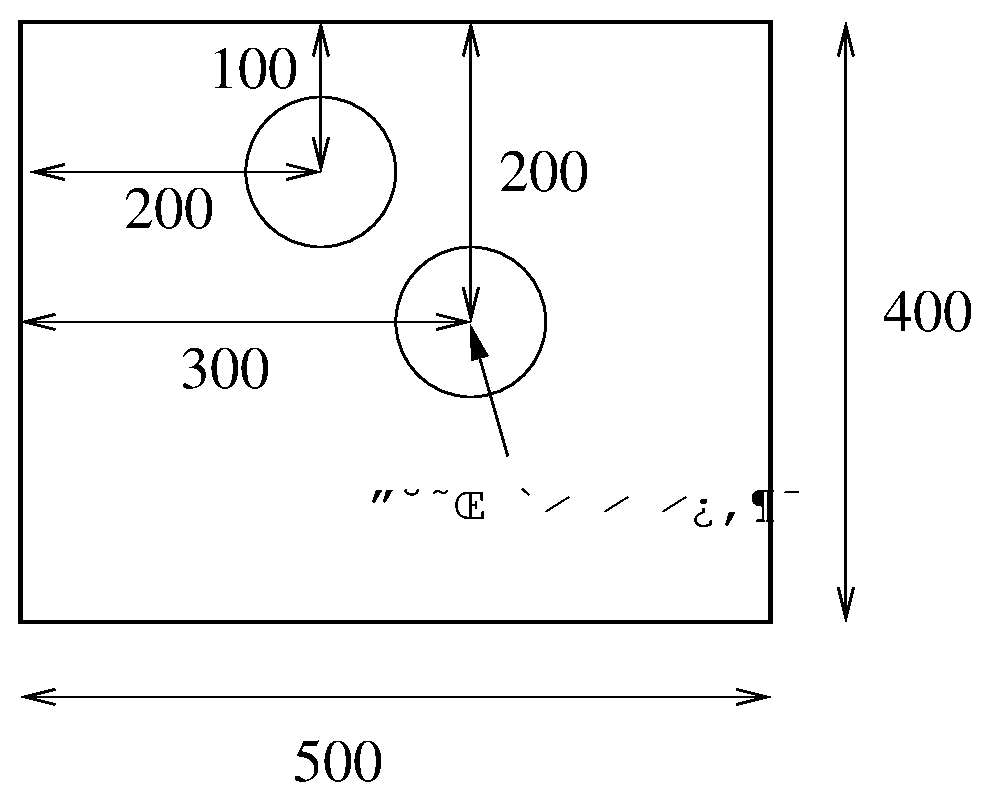
\epsfig{file=./eps/gsetmaps01.eps, width=2.0in}
\caption{$\!\!\!\!$\colorbox{white}{{\textcolor{white}{:}}}}
\label{fig:gsetmaps01}
\end{center}
%\end{figure}
\end{minipage}
\end{center}
\end{figure}
   \end{quotation}
\end{enumerate2}

% (4) サンプルプログラム
% \begin{enumerate2}
% \item {\bf{sample1}}
% \begin{center}
% \begin{table}[!h]
% \begin{tabular}{ll}
% \multicolumn{2}{l}{/* 内部を塗りつぶした矩形を描くプログラム */} \\
% gOpenWindow(400, 400)         & /* 横400、縦400のwindowを開く */ \\
% gSetLineColor(0, 0, 255)      & /* 線の色を青の要素255に設定する */ \\
% gSetFillColor(0, 220, 0)      & /* 図形内部の色を緑の要素220に設定する */ \\
% gFillBox(100, 120, 200, 140)  & /* 矩形を(100, 120)に 幅200、高さ140で描く */ 
% \end{tabular}
% \end{table}
% \end{center}
% 
% \item {\bf{sample2}} \\
% \begin{center}
% \begin{table}[!h]
% \begin{tabular}{ll}
% \multicolumn{2}{l}{/* 日本の国旗を描くプログラム */} \\
% gOpenWindow(400, 400)       & /* 横400、縦400のwindowを開く。 */ \\
% gSetFillColor(255, 0, 0)    & /* 図形内部の色を赤の要素255に設定する。 */ \\
% gFillCircle(200, 200, 40)   & /* (200, 200)を中心に、半径40の円を描く。 */ \\
% gDrawBox(80, 120, 240, 160) & /* 矩形を(80, 120)に、幅240、高さ160で描く */ \\
% gSetFontSize(40)            & /* 文字の大きさを40に設定する。 */ \\
% gDrawText("日本", 160, 320) & /* 「日本」と(160, 320)から描く。 */ \\
% \end{tabular}
% \end{table}
% \end{center}
% \end{enumerate2}

\newpage

\begin{center}
\begin{LARGE}
{\bf{(補足)~グラフ描画のための関数群\\
\ \\}}
\end{LARGE}
\end{center}

 このドキュメントは、PENの描画機能を用いて、主として2次元座標
平面上でグラフを描画するためのものである。
描画ウィンドウを開くためにはgOpenWindow()の代わりに
gOpenGraphWindow()関数を用いる。
これによって、2次元仮想平面上の任意の矩形領域を描画ウィンドウに
マッピングすることができる。
以後の描画命令は、仮想平面に対して『図形描画のための関数群』を
そのまま利用することができる。

gSetMap()関数は、仮想平面上の原点の並行移動もしくは、仮想平面上
の任意の矩形領域を描画ウィンドウに再マッピングするためのものである。

%  グラフ描画のための関数は以下の関数群から構成される。
%\begin{itemize2}
%  \item [(1)] 描画のためのウィンドウのオープン/クローズ関数 
%  \item [(2)] 図形の属性を指定するための関数 
%  \item [(3)] 図形を描画するための関数 
%\end{itemize2}
%
%  図形は、一つのウィンドウ上に描画する。このウィンドウの大きさを指定し
%て開くための関数として gOpenGraphWindow()がある。 gCloseWindow()は閉じるた
%めの関数であるが、この関数を呼び出すと描画ウィンドウが画面から消滅す
%るので、通常gCloseWindow()を使用することはない。 \\
%  図形は、線分、折れ線などの{\bf{線図形}}、長方形、楕円、
%多角形などの{\bf{面図形}}、
%および、{\bf{文字図形}}からなる。 図形を描くには、原則として先に描画属性を指 
%定しなければな らない。描画属性としては、線の太さ、線の種類、線の色等 
%の線図形に適応されるもの、塗りつぶしの色等の面図形に適応されるもの、 
%および、フォントの種類、フォントサイズ等の文字図形に適応されるものが 
%ある。描画属性を指定しない場合は、予め定められた属性値が用いられ、一 
%旦、設定した属性値は、同じ属性に対して新たに設定されるまで有効である。 
%  図形を描画するための関数としてここでは、多角形の描画の関数を示す。 \\
%
%  以下、各関数について説明する。

%(1) グラフ描画のためのウィンドウのオープン/クローズ関数 
グラフ描画のためのウィンドウのオープン/クローズ関数 

\begin{enumerate2}
\item {\bf{gOpenGraphWindow(実数 width, 実数 height, 実数 x1, 実数 y1, 実数 x2, 実数 y2, 論理値 axis)}} \\
%   \ \ 実数  width, height, x1, x2, y1, y2  \\
%   \ \ 論理値 axis
\vspace{-5mm}
   \begin{quotation}
   幅 width、高さ height の描画ウィンドウを開く。
   ウィンドウの左下を(x1,y1)座標とし、右上を(x2, y2)座標
   となるような座標平面として定義する。
   axis の値を true, false に指定することで座標軸の表示、非表示を指定する。
   \end{quotation}
   \begin{quotation}
\begin{figure}[!h]
\begin{center}
\begin{minipage}{24zw}
	   \noindent $[$使用例$]$\\
\ \\
幅500、高さ500の描画ウィンドウを用意し、
そのウィンドウの左下を(-50, -100)、右上を(350,300)の仮想座標空間として定義する。
また、xy座標軸を表記する。(図~\ref{fig:gopengraphwindow}) \\

{\small{gOpenGraphWindow(500, 500, -50, -100, 350, 300, true)}}
\end{minipage}
\begin{minipage}{20zw}
%\begin{figure}[!h]
\begin{center}
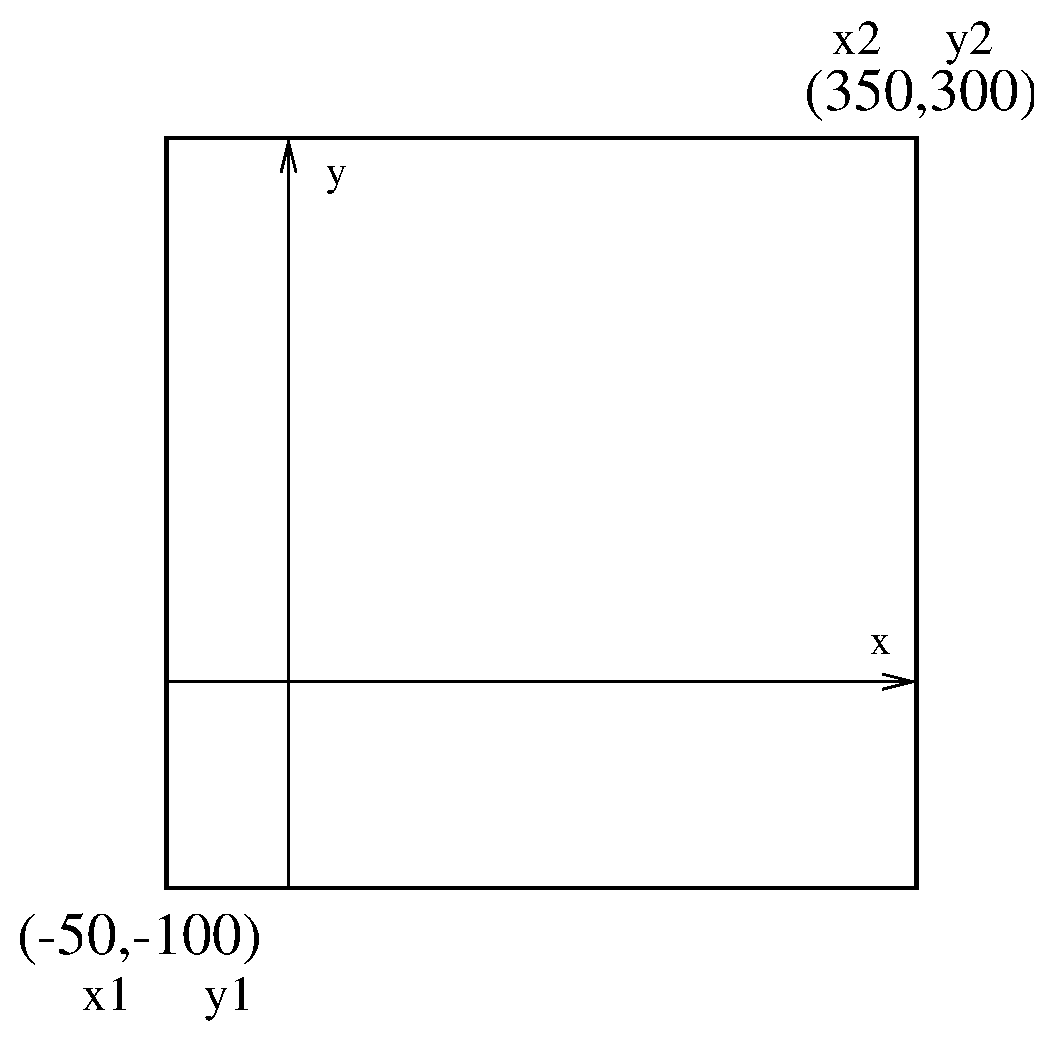
\epsfig{file=./eps/gopengraphwindow.eps, width=1.9in}
\caption{$\!\!\!\!$\colorbox{white}{{\textcolor{white}{:}}}}
%\caption{gOpenGraphWindowの例}
\label{fig:gopengraphwindow}
\end{center}
%\end{figure}
\end{minipage}
\end{center}
\end{figure}
   \end{quotation}


\item {\bf{gSetMap(実数x1, 実数y1, 実数x2, 実数y2)}} \\
%  \ \    実数 x1, x2, y1, y2
  \begin{quotation}
     描画ウィンドウの左下を点(x1,y1)、右上を点(x2,y2)として再指定する。
     (図~\ref{fig:gsetmaps02})\\
  \end{quotation}
\begin{quotation}
\begin{figure}[!h]
\begin{minipage}{25zw}
\noindent $[$使用例$]$ \\

図~\ref{fig:gopengraphwindow}のウィンドウを開いた後、
左下を(0,-50)、右上を(150,200)の座標空間として再定義する。\\


{\small{
 gOpenGraphWindow(500, 500, -50, -100, 350, 300, true) \\
 gSetMap(0, -50, 150, 200) \\
}}
\end{minipage}
\begin{minipage}{20zw}
%\begin{figure}[!h]
\begin{center}
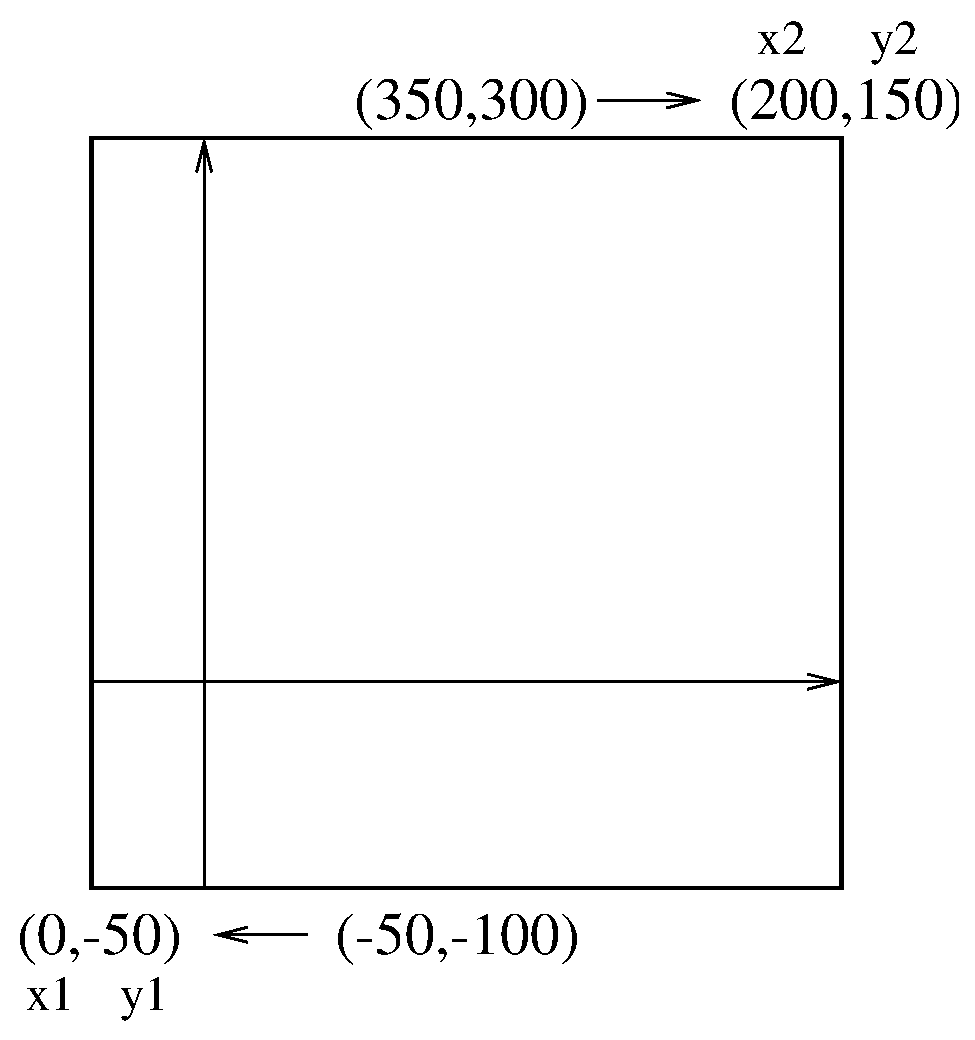
\epsfig{file=./eps/gsetmaps02.eps, width=2.0in}
\caption{$\!\!\!\!$\colorbox{white}{{\textcolor{white}{:}}}}
\label{fig:gsetmaps02}
\end{center}
%\end{figure}
\end{minipage}
\end{figure}
   \end{quotation}
\end{enumerate2}

\end{document}

%%%xDNCL-draw.tex へ移動
%%% gSetMap --> gSetOrigin へ名称変更(の予定)
%%%
\item {\bf{gSetDrawArea(実数x, 実数y)}} \\
%   \ \  実数 x, y 
\vspace{-5mm}
   \begin{quotation}
     描画ウィンドウの左上からの右方向にx、下方向にyの点を原点として再定義する。
   \end{quotation}
   \begin{quotation}
\begin{figure}[!h]
\begin{center}
\begin{minipage}{25zw}
	   \noindent $[$使用例$]$\\

\noindent 図~\ref{fig:gopengraphwindow}の描画ウィンドウの
(100,150)を中心とする円(r=50)を描いた後に、この座標空間の(100,0)を原点に再定義する。
そして、再定義した原点を中心とする円(r=50)を描く。(図~\ref{fig:gsetmaps01})
\ \\

{\small{
          gOpenGraphWindow(500, 500, -50, 350, -100, 300, true)\\
          gSetLineColor(255, 0, 0)  \\
          gDrawCircle(100, 150, 50)  \\
          gSetDrawArea(150, 300) \\
          gSetLineColor(0, 255, 0)  \\
          gDrawCircle(0, 0, 50)  \\
}}
\end{minipage}
\begin{minipage}{20zw}
%\begin{figure}[!h]
\begin{center}
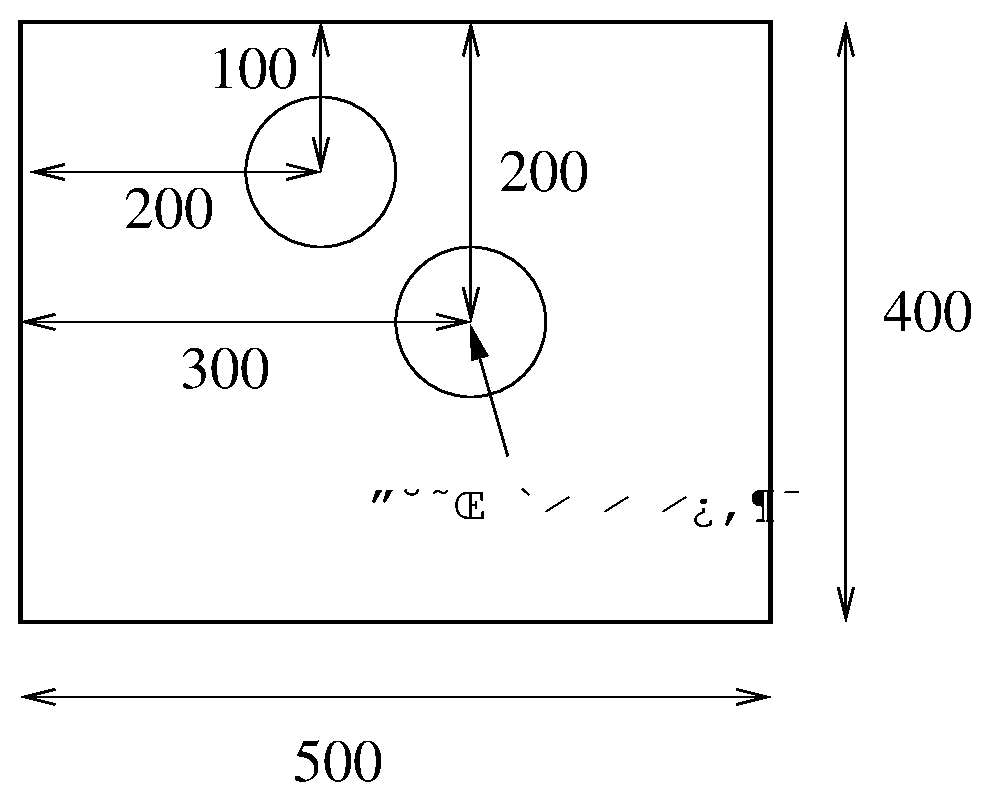
\epsfig{file=./eps/gsetmaps01.eps, width=2.0in}
\caption{$\!\!\!\!$\colorbox{white}{{\textcolor{white}{:}}}}
\label{fig:gsetmaps01}
\end{center}
%\end{figure}
\end{minipage}
\end{center}
\end{figure}
   \end{quotation}


\end{document}


